\section{Xây dựng ứng dụng Android với React Native}

\subsection{Thiết lập môi trường}
Để bắt đầu xây dựng một ứng React Native, ta cần cài đặt môi trường lập trình trên thiết bị của mình. Cụ thể cần: NodeJS, JDK, Android Studio.
\subsubsection{NodeJS}
\begin{enumerate}
    \item[\textit{a.}] {\textit{Tổng quan}}\\
    NodeJS là một nền tảng (flatform) cung cấp môi trường runtime chạy JavaScript, được sử dụng để chạy các ứng dụng web bên ngoài client. Nền tảng này được phát triển bởi Ryan Dahl vào năm 2009, được xem là một giải pháp hoàn hảo cho các ứng dụng sử dụng nhiều dữ liệu nhờ vào mô hình hướng sự kiện (event-driven) không đồng bộ.
    NodeJS cung cấp các package để xây dựng ứng dụng React Native.
    \item[\textit{b.}] {\textit{Cài đặt}}\\
    Link cài đặt: \url{https://nodejs.org/en/download/}\\
    Có thể cài bằng các dòng lệnh thông qua terminal (phụ thuộc vào hệ điều hành của thiết bị):
    \begin{enumerate}
        \item[-] {Windows}: choco install -y nodejs-lts
        \item[-] {MacOS}: brew install node | brew install watchman
        \item[-] {Linux}: apk add nodejs npm
    \end{enumerate}
    Sau khi cài đặt xong, có thể kiểm tra lại bằng cách chạy dòng lệnh trong terminal:
    \begin{figure}[!ht]
        \centering
        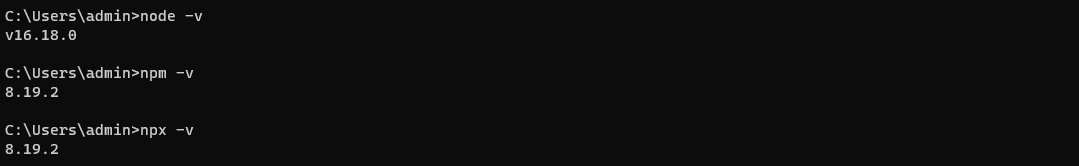
\includegraphics[width=1\textwidth]{images/checkNodeJS.png}
        \caption{Cài đặt NodeJs}
    \end{figure}
\end{enumerate}
\subsubsection{JDK}
\begin{enumerate}
    \item[\textit{a.}] {\textit{Tổng quan}}\\
    JDK (Java Development Kit) là một trong ba gói công nghệ cốt lõi được sử dụng trong lập trình Java: JVM (Máy ảo Java - Java Virtual Machine), JRE (Java Runtime Enviroment - Môi trường Java Runtime), JDK.\\
    Có thể định nghĩa JDK theo 2 cách sau:
    \begin{enumerate}
        \item[-] {\textit{Định nghĩa chuyển ngành}}: JDK là một hệ tiêu chuẩn trong việc triển khai nền tảng Java, bao gồm các trình thông dịch và thư viện lớp.
        \item[-] {\textit{Định nghĩa thông thường}}: JDK là gói phần mềm bạn tải xuống để tạo các ứng dụng dựa trên Java.
    \end{enumerate}
    Như đã trình bày ở phần kiến trúc Android, tầng Android Runtime cần trình biên dịch Java để compile ra các lớp.
    \item[\textit{b.}] {\textit{Cài đặt}}\\
    Link cài đặt: \url{https://www.oracle.com/eg/java/technologies/downloads/}\\
    Có thể cài bằng các dòng lệnh thông qua terminal (phụ thuộc vào hệ điều hành của thiết bị):
    \begin{enumerate}
        \item[-] {Windows}: choco install -y microsoft-openjdk11
        \item[-] {MacOS}: brew install java
        \item[-] {Linux}: sudo apt install default-jdk
    \end{enumerate}
    Sau khi cài đặt xong, có thể kiểm tra lại bằng cách chạy dòng lệnh trong terminal:
    \begin{figure}[!ht]
        \centering
        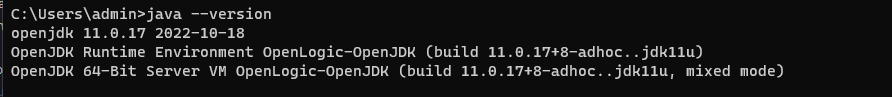
\includegraphics[width=1\textwidth]{images/checkJDK.png}
        \caption{Cài đặt JDK}
    \end{figure}
\end{enumerate}
\subsubsection{Android Studio}
\begin{enumerate}
    \item[\textit{a.}] {\textit{Tổng quan}}\\
    Android Studio là Môi trường phát triển tích hợp (IDE) chính thức để phát triển ứng dụng Android.\\
    Nhờ các công cụ cho nhà phát triển tích hợp trình soạn thảo mạnh mẽ của  \href{https://www.jetbrains.com/idea/}{IntelliJ IDEA}, Android Studio cung cấp các tính năng giúp hỗ trợ và nâng cao năng suất trong quá trình phát triển ứng dụng Android:
    \begin{enumerate}
        \item[-] Hệ thống xây dựng linh hoạt dựa trên Gradle.
        \item[-] Trình mô phỏng nhanh và có nhiều tính năng.
        \item[-] Môi trường hợp nhất để phát triển các thiết bị Android.
        \item[-] Tự cập nhật thay đổi ứng dụng mà đang chạy mà không cần khởi động lại.
        \item[-] Hỗ trợ tự động chạy code template và code snippet.
        \item[-] Tích hợp GitHub để tạo môi trường làm việc hiệu quả.
    \end{enumerate}
    \item[\textit{b.}] {\textit{Cài đặt}}\\
    Link cài đặt: \url{https://developer.android.com/studio}\\
    Trong quá trình cài đặt Android Studio cần đảm bảo có các mục được chọn:
    \begin{enumerate}
        \item[-] Android SDK.
        \item[-] Android SDK Platform.
        \item[-] Android Virtual Device.
    \end{enumerate}
    Sau khi cài đặt Android Studio, cần cấu hình Android SDK phù hợp để chạy React Native (theo yêu cầu được cung cấp trong tài liệu). Cụ thể, trong Android Studio, chọn "Appearance \char`& Behavior" -> "System setting" -> "Android SDK". Khi đó cần cài các gói:
    \begin{enumerate}
        \item[-] SDK Flatform: Android SDK Platform 33, Intel x86 Atom\char`_64 System Image.
        \item[-] SDK Tools: Android SDK Build-Tools 33.0.0.
    \end{enumerate}
    Một yêu cầu khác, các công cụ React Native yêu cầu biến môi trường được thiết lập để code. Cụ thể, cần cấu hình biến ANDROID\char`_HOME cho đường dẫn SDK Android và thêm đường dẫn SDK Android Flatform vừa cài đặt trên (cụ thể phụ thuộc vào hệ điều hành của thiết bị).
    \begin{figure}[!ht]
        \centering
        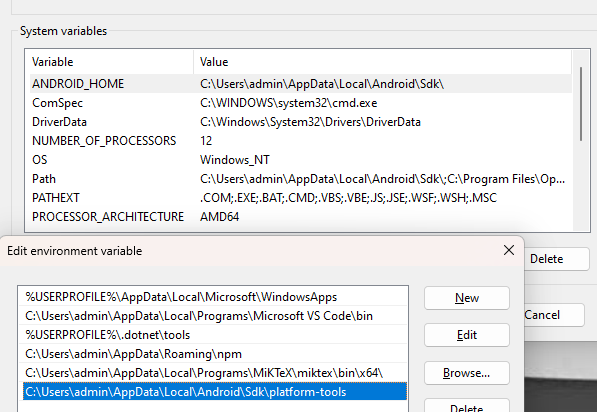
\includegraphics[scale=0.5]{images/configVariable.png}
        \caption{Cài đặt biến môi trường ANDROID\char`_HOME}
    \end{figure}
\end{enumerate}

\subsection{Xây dựng chương trình đầu tiên}
Nếu trước đó thiết bị đã cài đặt gói react-native-cli toàn cầu, chúng ta cần xóa gói này vì gói đó có thể gây ra các sự cố không mong muốn:
\begin{figure}[!ht]
    \centering
    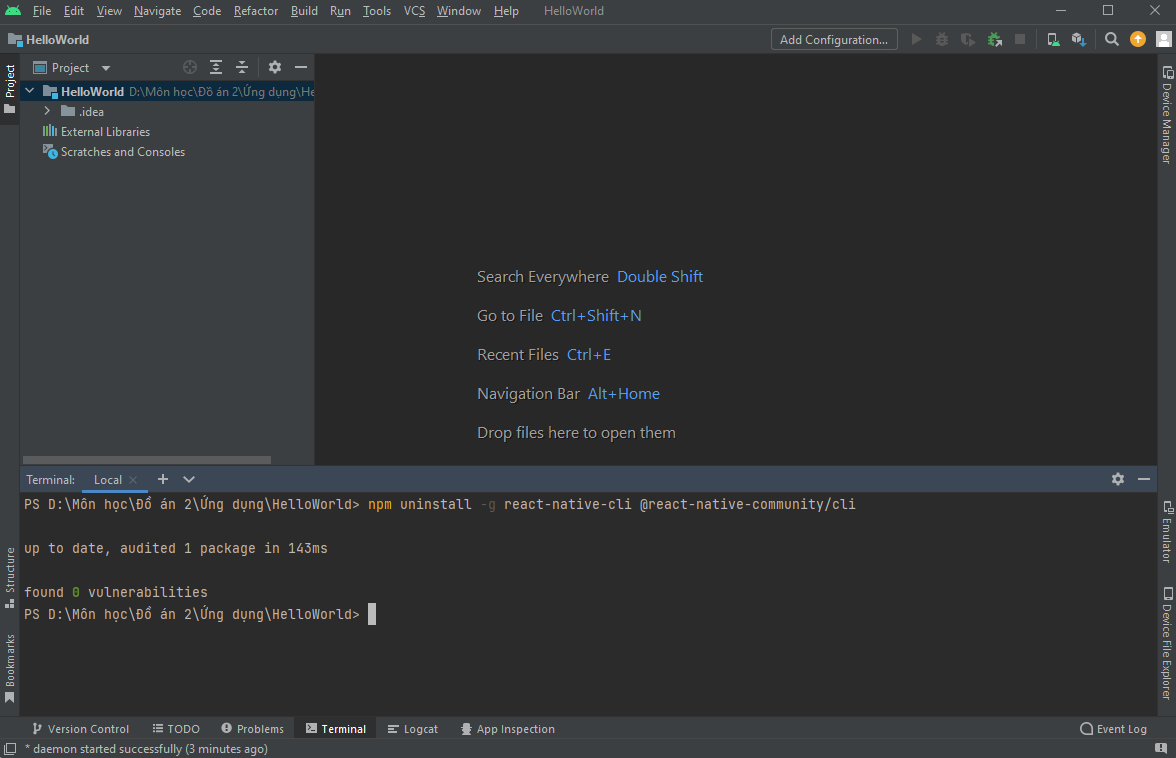
\includegraphics[width=1\textwidth]{images/deleteReactnativeCLI.png}
    \caption{Xoá gói React Native CLI}
\end{figure}

Để bắt đầu xây dựng chương trình, ta tạo thư mục cho project này. Cụ thể, tôi đặt "HelloWorld". Sau đó mở thư mục đó bằng Android Studio, chạy dòng lệnh sau trên terminal:
\begin{figure}[!ht]
    \centering
    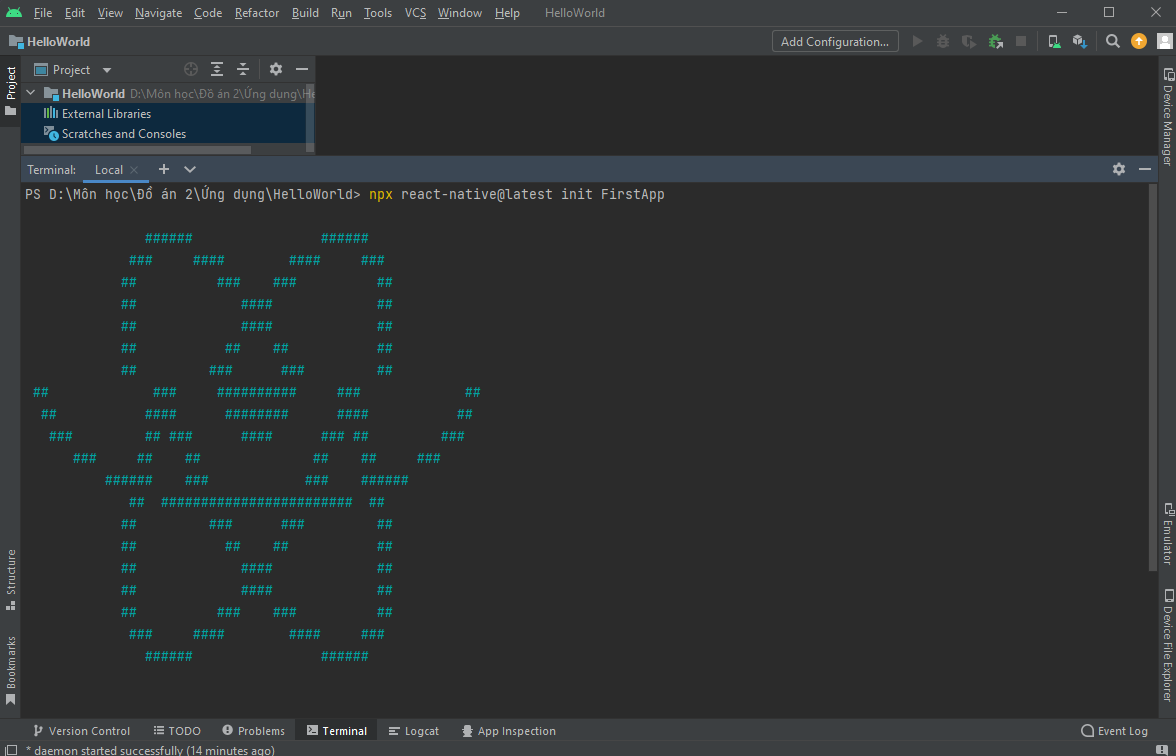
\includegraphics[width=1\textwidth]{images/createFirstApp.png}
    \caption{Khởi tạo ứng dụng React Native}
\end{figure}

Cụ thể, "npx" là công cụ CLI do NodeJs cung cấp để cài đặt và quản lý các thành phần phụ thuộc npm. Ta sử dụng gói react-native để khởi tạo ứng dụng FirstApp.
Sau khi chạy dòng lệnh trên, quan sát project, ta thấy thư mục FirstApp và các file trong đó:
\begin{figure}[!ht]
    \centering
    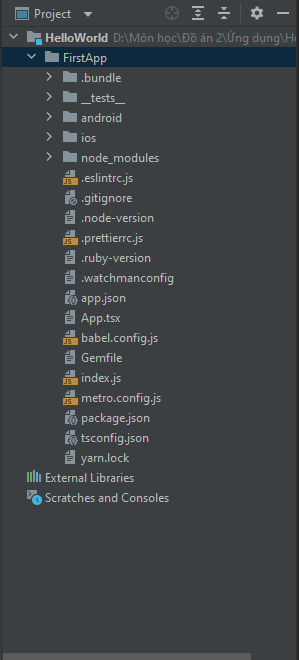
\includegraphics[scale=0.5]{images/firstAppData.png}
    \caption{Dữ liệu FirstApp}
\end{figure}
\newline
Công việc tiếp theo là chạy ứng dụng FirstApp đã khởi tạo trên. Có 2 cách để build và chạy ứng dụng react native trong quá trình xây dựng:
\begin{enumerate}
    \item[-] Chạy trên thiết bị vật lý
    \item[-] Chạy trên máy ảo
\end{enumerate}

\subsubsection{Chạy trên thiết bị vật lý}
\begin{enumerate}
    \item[\textit{a.}] {\textit{Bật gỡ lỗi trên thiết bị vậy lý}}\\
    Để bật gỡ lỗi trên thiết bị Android của bạn, ta cần thực hiện các bước:
    \begin{enumerate}
        \item[-] Bật chế độ nhà phát triển
        \item[-] Bật gỡ lỗi USB
    \end{enumerate}
    Cụ thể cách bật chế độ nhà phát triển sẽ khác nhay tùy thuộc vào thiết bị, có thể tìm kiếm cách bật trên trình duyệt. Tuy nhiên để bật chế độ này có thể tổng quát: \textbf{Cài đặt} → \textbf{Giới thiệu về điện thoại} → \textbf{Thông tin phần mềm} rồi nhấn Build number bảy lần vào hàng ở dưới cùng; sau đó, quay lại \textbf{Cài đặt} → \textbf{Tùy chọn nhà phát triển} để bật "Gỡ lỗi USB".
    \item[\textit{b.}] {\textit{Kết nối với thiết bị}}\\
    Tiếp theo cần kết nối thiết bị Android với thiết bị phát triển ứng dụng qua USB. Sau đó, kiểm tra lại thiết bị đã bật gỡ lỗi USB chưa bằng cách chạy dòng lệnh "adb devices".
    \begin{figure}[!ht]
        \centering
        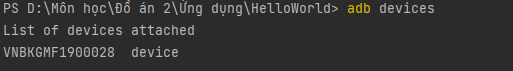
\includegraphics[width=1\textwidth]{images/checkDevices.png}
        \caption{Kiểm tra kết nối thiết bị}
    \end{figure}
    \item[\textit{c.}] {\textit{Chạy ứng dụng trên thiết bị}}\\
    Để chạy ứng dụng, ta di chuyển đến FirstApp và chạy dòng lệnh sau: npx react-native run-android.
    % Ảnh build chạy trên thiết bị
\end{enumerate}
\subsubsection{Chạy trên máy ảo}
\begin{enumerate}
    \item[\textit{a.}] {\textit{Tạo AVD mới}}\\
    Trước hết ta cần tạo AVD mới bằng Android Studio. Ta vào mục \textbf{Device Manager} → \textbf{Create device}
    \begin{figure}[!ht]
        \centering
        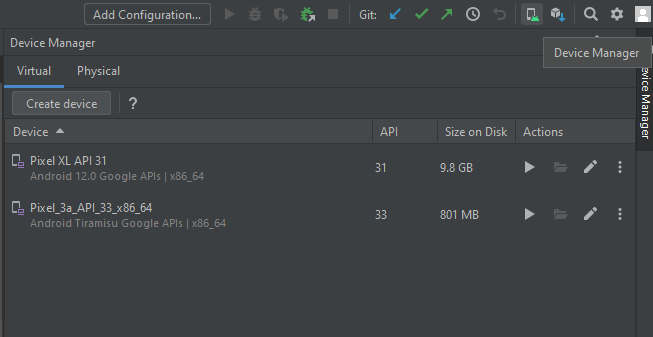
\includegraphics[width=1\textwidth]{images/createAVD.png}
        \caption{Tạo thiết bị ảo trên Android Studio}
    \end{figure}
    Sau đó, Android Studio hiển thị giao diện cấu hình thiết bị, ta chọn bất kỳ Điện thoại nào từ danh sách và nhấp vào \textbf{Next}, sau đó chọn hình ảnh \textbf{Tiramisu} API Cấp 33. Tiếp theo chọn \textbf{Finish} để tạo thiết bị ảo.
    \item[\textit{b.}] {\textit{Kiểm tra kết nối}}\\
    Sau khi khởi tạo, ta mở thiết bị ảo trên Android Studio và kiểm tra (giống chạy trên thiết bị vật lý):
    \begin{figure}[!ht]
        \centering
        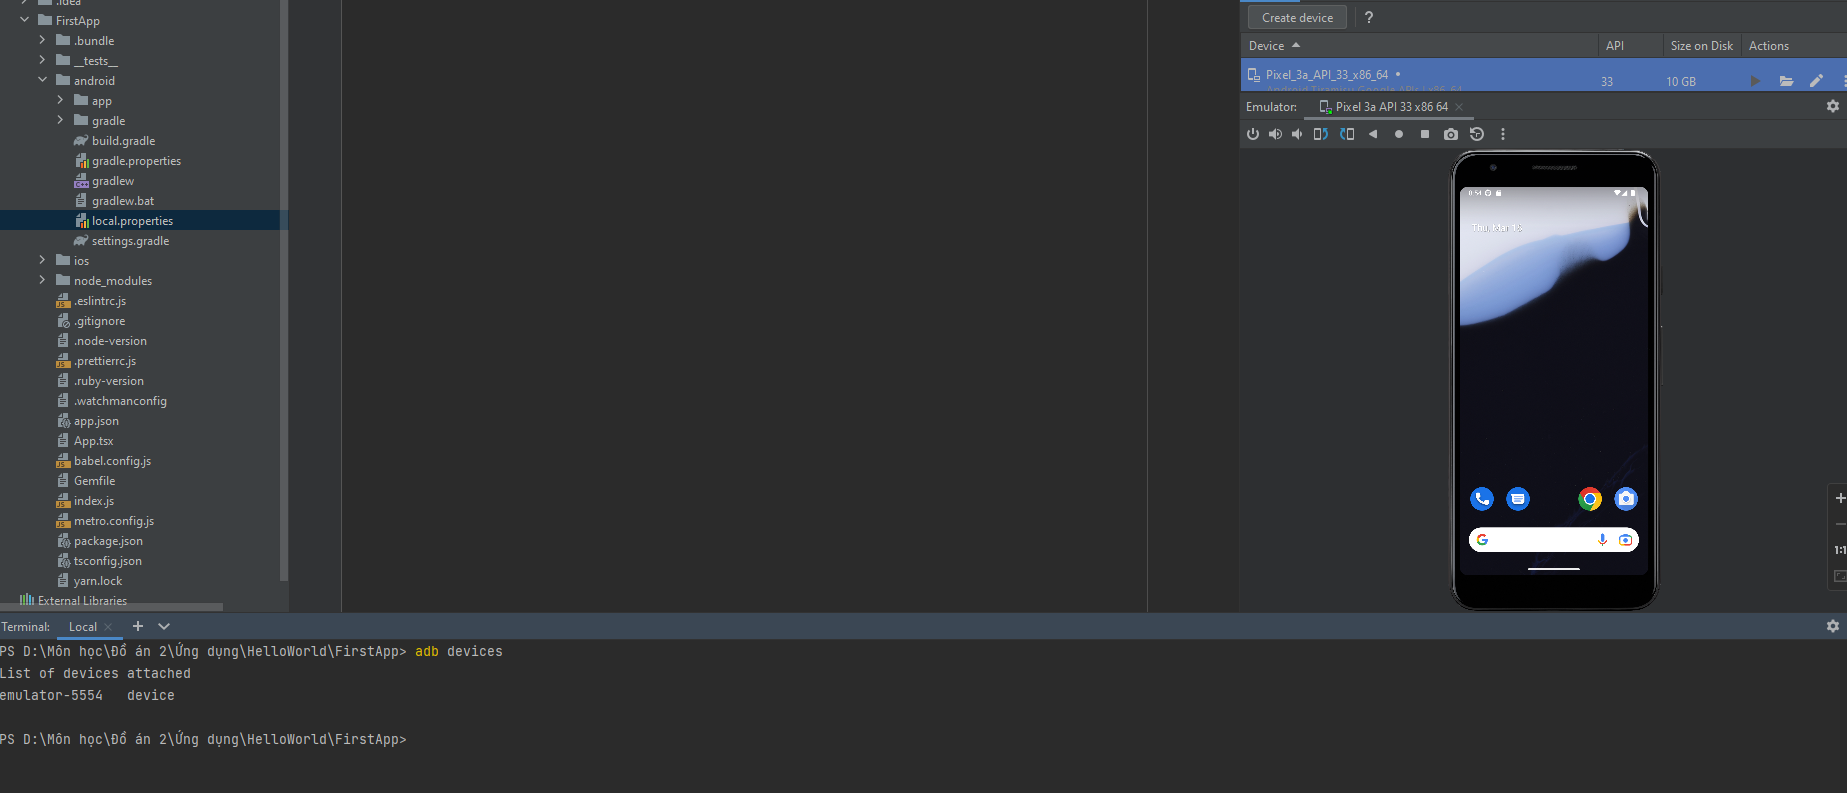
\includegraphics[scale=0.3]{images/runAVD.png}
        \caption{Kiểm tra kết nối thiết bị ảo trên Android Studio}
    \end{figure}
    \item[\textit{c.}] {\textit{Chạy ứng dụng trên AVD}}\\
    Thực hiện chạy ứng dụng trên thiết bị ảo giống trên thiết bị vật lý.
    % Ảnh build chạy trên thiết bị ảo
\end{enumerate}

\subsection{Các khái niệm, thành phần}
\subsubsection{Components}
Trong quá trình phát triển Android, người ta thường phân giao diện thành các khối hình chữ nhật để thực hiện các chức năng riêng như: hiển thị văn bản, hình ảnh, phản hồi của người dùng,\dots Mỗi một khối như vậy được gọi là View.
\begin{figure}[!ht]
    \centering
    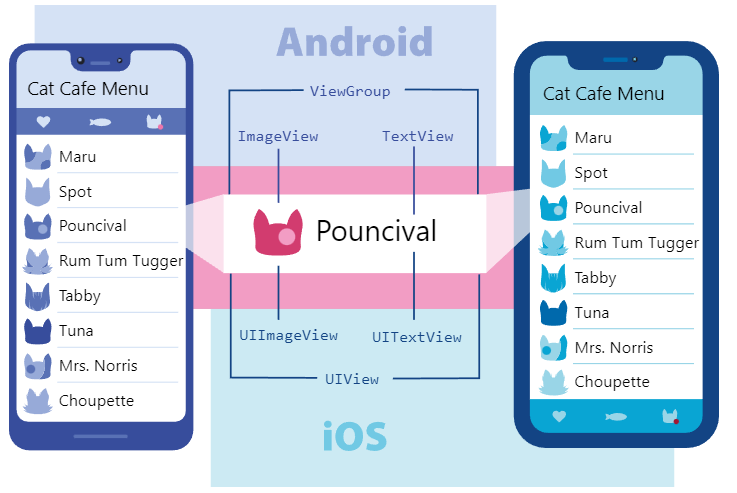
\includegraphics[scale=0.5]{images/nativeViewComponent.png}
    \caption{View trong giao diện Native}
\end{figure}
Đối với React Native, các View trên được gọi là \textit{Component}. Một cách dễ hiểu, để xây dựng ứng dụng React Native, ta cần tập chung mô tả giao diện mong muốn thành các component như trên.\\
Ta có thể phân loại các components như hình vẽ sau (chứa cả React Component vì React Native được xây dựng dựa trên ReactJS)
\begin{figure}[!ht]
    \centering
    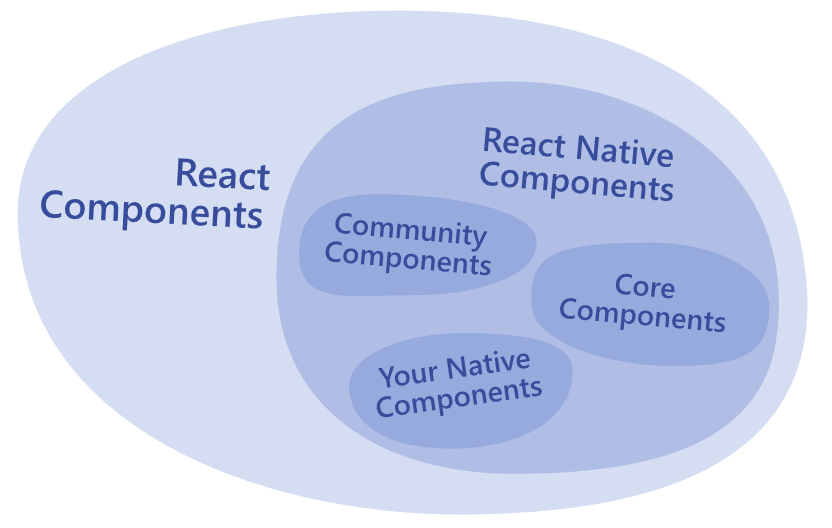
\includegraphics[scale=0.5]{images/reactComponents.png}
    \caption{Phân loại các component}
\end{figure}
\begin{enumerate}
    \item[\textit{a.}] {\textit{Core Components}}\\
    Core Components là các component cốt lõi để xây dựng ra các component khác. Các component này điều khiển các hành động cơ bản về giao diện như: hiển thị văn bản, hình ảnh, cho phép người dùng nhập, ấn,\dots\\
    \begin{figure}[!ht]
        \centering
        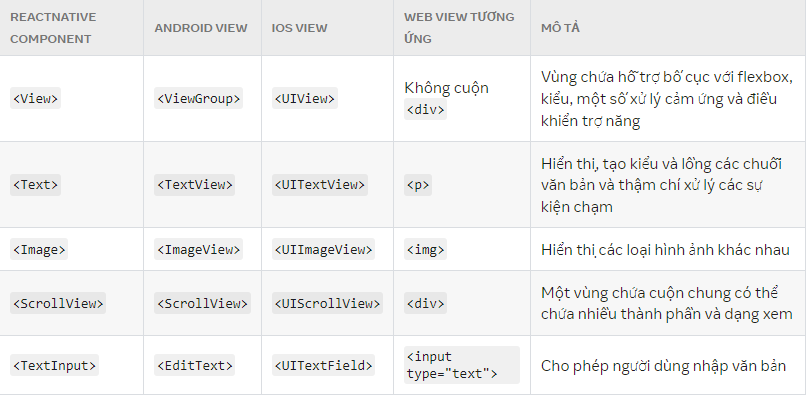
\includegraphics[width=1\textwidth]{images/coreComponets.png}
        \caption{Mô tả một số Core Components}
    \end{figure}
    Có thể phân loại Core Component như sau:
    \begin{enumerate}
        \item[-] {\textit{Basic Components}}: bao gồm các component trong bảng 13.
        \item[-] {\textit{User Interface}}: Gồm các component điều khiển các hành động của người dùng:
        \begin{enumerate}
            \item[+] Button: Xử lý thao tác chạm của người dùng.
            \item[+] Switch: Xử lý bật/tắt cho một chức năng.
        \end{enumerate}
        \item[-] {\textit{List View}}: Không giống như ScrolView, các component này hiển thị nội dung dưới dạng các phần tử. Điều này làm cho chúng trở thành lựa chọn hiệu quả để hiển thị danh sách dữ liệu dài. Bao gồm:
        \begin{enumerate}
            \item[+] FlatList: Hiển thị một danh sách có thể cuộn.
            \item[+] SectionList: Giống FlatList nhưng đối với danh sách được phân đoạn.
        \end{enumerate}
        \item[-] {\textit{Android-specific}}: là các component cung cấp các dịch vụ đặc trưng của Android. Bao gồm:
        \begin{enumerate}
            \item[+] BackHandler: Phát hiện các nút phần cứng điều hướng quay lại. (Ví dụ: nút back ảo, vuốt cạnh bên,\dots)
            \item[+] DrawerLayoutAndroid: Tạo một giao diện dạng ngăn kéo trên Android.
            \item[+] PermissionsAndroid: Cung cấp quyền truy cập đối với Android
            \item[+] ToastAndroid: Tạo một cảnh báo trên Android
        \end{enumerate}
        \item[-] {\textit{iOS-specific}}: là các component cung cấp các dịch vụ đặc trưng của UIKit. (Đồ án này chỉ tìm hiểu về react native và android nên không đi sâu vào IOS, chỉ nêu ra ở đây) 
        \item[-] {\textit{Other}}: các component thường dùng khác
        \begin{enumerate}
            \item[+] ActivityIndicator: Hiển thi giao diện loading xoay tròn
            \item[+] Alert: Hiển thị hộp thoại thông báo với tiêu đề và nội dung
            \item[+] Animated: Một thư viện để tạo các hoạt ảnh linh hoạt, mạnh mẽ, dễ xây dựng và bảo trì.
            \item[+] Dimensions: Cung cấp giao diện để nhận kích thước thiết bị.
            \item[+] KeyboardAvoidingView: Cung cấp giao diện điều khiển hiển thị bàn phím.
            \item[+] Linking: Xử lý hành động tương tác với liên kết.
            \item[+] Modal: Một giao diện nổi phía trên giao diện gốc.
            \item[+] PixelRatio: Cung cấp quyền truy cập vào mật độ pixel của thiết bị.
            \item[+] RefreshControl: Thành phần này được sử dụng bên trong ScrollView chức năng thêm kéo để làm mới.
            \item[+] StatusBar: Thành phần để kiểm soát thanh trạng thái ứng dụng.
        \end{enumerate}
    \end{enumerate}
    Các core component được cung cấp trong package "react-native", vì thế để sử dụng chúng, ta chỉ cần import từ package đó:
    \begin{figure}[!ht]
        \centering
        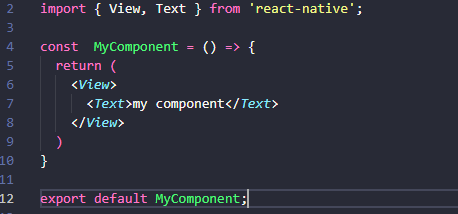
\includegraphics[width=1\textwidth]{images/coreComponetExample.png}
        \caption{Ví dụ sử dụng Core Component}
    \end{figure}
    \item[\textit{b.}] {\textit{Community Components}}\\
    Như đã trình bày, cộng đồng phát triển React Native rất lớn, vì thế để phục vụ cho phát triển ứng dụng nhanh chóng, một số nhóm, công ty xây dựng ra các gói, thư viện chứa các component xây dựng sẵn như: ant-design, axios, calendar, react-native-webview,\dots Cụ thể các thư viện này được trình bày tại mục "Một số thư viện phổ biến".\\
    Để sử dụng được các component này, ta cần cài đặt các thư viện bằng dòng lệnh: npm install <package-name>
    \begin{figure}[!ht]
        \centering
        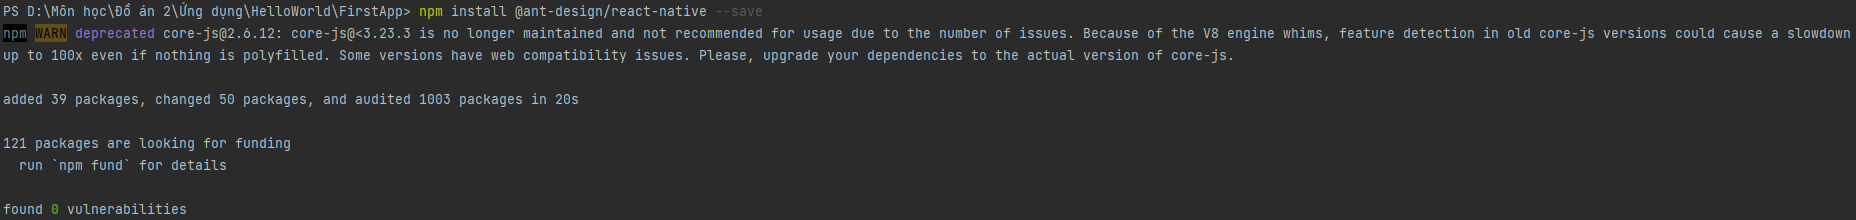
\includegraphics[width=1\textwidth]{images/installPackage.png}
        \caption{Cài đặt package - AntDesign}
    \end{figure}
    Sau khi cài đặt gói thành công, các component này sử dụng như core component, chỉ cần import và sử dụng.
    \item[\textit{c.}] {\textit{Your Native Components}}\\
    Đây là các component do chính người phát triển ứng dụng xây dựng.\\
    Việc phân chia, xây dựng các component một các chính xác giúp cho ứng dụng được tối ưu, tái sử dụng code một cách hiệu quả
\end{enumerate}
\subsubsection{JSX}
\subsubsection{Props}
\subsubsection{State}

\subsection{Một số thư viện phổ biến}

\subsection{Phát hành ứng dụng}
